\documentclass[submit]{harvardml}

\course{CS181-S24}
\assignment{Assignment \#2}
\duedate{11:59pm EST, Feb 23th, 2024}

\usepackage[OT1]{fontenc}
\usepackage[colorlinks,citecolor=blue,urlcolor=blue]{hyperref}
\usepackage[pdftex]{graphicx}
\usepackage{subfig}
\usepackage{fullpage}
\usepackage{amsmath}
\usepackage{amssymb}
\usepackage{framed}
\usepackage{color}
\usepackage{soul}
\usepackage{todonotes}
\usepackage{listings}
\usepackage{common}
\usepackage{enumitem}
\usepackage{bm}
\usepackage{bbm}
\newcommand{\B}{\text{B}}
\newcommand{\Beta}{\text{Beta}}

\usepackage[mmddyyyy,hhmmss]{datetime}

\definecolor{verbgray}{gray}{0.9}

\lstnewenvironment{csv}{%
  \lstset{backgroundcolor=\color{verbgray},
  frame=single,
  framerule=0pt,
  basicstyle=\ttfamily,
  columns=fullflexible}}{}




\begin{document}

\begin{center}
{\Large Homework 2: Classification and Bias-Variance Trade-offs}\\
\end{center}

\subsection*{Introduction}

This homework is about classification, bias-variance trade-offs, and
uncertainty quantification.

The datasets that we will be working with relate to astronomical
observations. The first dataset, found at \verb|data/planet-obs.csv|,
contains information on whether a planet was observed (as a binary
variable) at given points in time. This will be used in Problem 1. The
second dataset, available at \verb|data/hr.csv|, details different
kinds of stars and their measured magnitude and temperature. You will
work with this data in Problem 3.

As a general note, for classification problems we imagine that we have
the input matrix $\boldX \in \reals^{n \times d}$ (or perhaps they
have been mapped to some basis $\bm{\Phi}$, without loss of
generality) with outputs now ``one-hot encoded."  This means that if
there are~$K$ output classes, rather than representing the output
label $y$ as an integer~${1,2,\ldots,K}$, we represent $\boldy$ as a
``one-hot" vector of length~$K$. A ``one-hot" vector is defined as
having every component equal to 0 except for a single component which
has value equal to 1.  For example, if there are $K = 7$ classes and a
particular data point belongs to class 3, then the target vector for
this data point would be~$\boldy = [0,0,1,0,0,0,0]$.  We will define
$C_1$ to be the one-hot vector for the 1st class, $C_2$ for the 2nd
class, etc.  Thus, in the previous example $\boldy = C_3$. If there
are $K$ total classes, then the set of possible labels is $\{C_1
\ldots C_K \} = \{C_k\}_{k=1}^K$.  Throughout the assignment we will
assume that each label $\boldy \in \{C_k\}_{k=1}^K$ unless otherwise
specified. The most common exception is the case of binary
classification ($K = 2$), in which case labels are the typical
integers $y \in \{0, 1\}$.

\subsection*{Resources and Submission Instructions}

We encourage you to read CS181 Textbook's Chapter 3 for more
information on linear classification, gradient descent, and
classification in the discriminative setting. Read Chapter 2.8 for
more information on the trade-offs between bias and variance.

In problems 1 and 3, you may use \texttt{numpy} or \texttt{scipy}, but
not \texttt{scipy.optimize} or \texttt{sklearn}. Example code is given
in the provided notebook.

Please type your solutions after the corresponding problems using this
\LaTeX\ template, and start each problem on a new page.

Please submit the \textbf{writeup PDF to the Gradescope assignment
  `HW2'}. Remember to assign pages for each question.  Please submit
your \textbf{\LaTeX\ file and code files to the Gradescope assignment
  `HW2 - Supplemental'}. \textbf{You must include your plots in your
  writeup PDF. } The supplemental files will only be checked in
special cases, e.g. honor code issues, etc.


%%%%%%%%%%%%%%%%%%%%%%%%%%%%%%%%%%%%%%%%%%%%%
% Problem 1
%%%%%%%%%%%%%%%%%%%%%%%%%%%%%%%%%%%%%%%%%%%%%

\begin{problem}[Exploring Bias-Variance and Uncertainty]
In this problem, we will explore the bias and variance of a few
different model classes when it comes to logistic regression and
investigate two sources of predictive uncertainty in a synthetic
(made-up) scenario.

We are using a powerful telescope in the northern hemisphere to gather
measurements of some planet of interest. At certain times however, our
telescope is unable to detect the planet due to its positioning around
its star.  The data in \verb|data/planet-obs.csv| records the
observation time in the ``Time" column and whether the planet was
detected in the ``Observed" column (with the value 1 representing that
it was observed).  These observations were taken over a dark, clear
week, which is representative of the region.  Since telescope time is
expensive, we would like to build a model to help us schedule and find
times when we are likely to detect the planet.

\begin{enumerate}
\item Split the data into 10 mini-datasets of size $N = 30$ (i.e. dataset 1 consists of the first 30 observations, dataset 2 consists of the next 30, etc. This has already been done for you). Consider the three bases $\boldsymbol\phi_1(t) = [1, t]$, $\boldsymbol\phi_2(t) = [1,
  t, t^2]$, and $\boldsymbol\phi_3(t) = [1, t, t^2, t^3, t^4, t^5]$. For each of these bases, fit a logistic regression model using sigmoid($\boldw^\top \boldsymbol\phi(t)$) to each dataset by using gradient descent to
  minimize the negative log-likelihood.  This means you will be
  running gradient descent 10 times for each basis, once for each
  dataset.
  
  Use the given starting values of $\boldw$ and a learning rate of $\eta=0.001$, take 10,000 update
  steps for each gradient descent run, and make sure to average the
  gradient over the data points at each step. These parameters,
  while not perfect, will ensure your code runs reasonably quickly. 

\item After consulting with a domain expert, we find that the probability of observing the planet is periodic as the planet revolves around its star---we are more likely to observe the planet when it is in front of its star than when it is behind it. In fact, the expert determines that observation follows the generating process $y \sim \text{Bern}(f(t))$, where $f(t) = 0.4 \times \cos(1.1t + 1) + 0.5$ for $t \in [0, 6]$ and $y \in \{0,1\}$. Note that we, the modelers, do not usually see the true data distribution. Knowledge of the true $f(t)$ is only exposed in this problem to allow for verification of the true bias.

Use the given code to plot the true process versus your learned models. Include your plots in your solution PDF.

\textbf{In no more than 5 sentences}, explain how bias and variance reflected in the 3 types of curves on the graphs.  How do the fits of the individual and mean prediction functions change?  Keeping in mind that none of the model classes match the true generating process exactly, discuss the extent to which each of the bases approximates the true process.

\end{enumerate}
\end{problem}

\newpage
\begin{framed}
\noindent\textbf{Problem 1} (cont.)\\
\begin{enumerate}
\setcounter{enumi}{2}

\item If we were to increase the size of each dataset drawn from $N = 30$ to a larger number, how would the bias and variance change for each basis? Why might this be the case? You may experiment with generating your own data that follows the true process and plotting the results, but this is \textbf{not} necessary. \textbf{Your response should not be longer than 5 sentences}.

\item Consider the test point $t = 0.1$. Using your models trained on basis $\boldsymbol\phi_3$, report the predicted probability of observation of the \textit{first} model (the model trained on the first 30 data points). How can we interpret this probability as a measure of uncertainty? Then, compute the variance of the classification probability over your 10 models at the same point $t = 0.1$. How does this measurement capture another source of uncertainty, and how does this differ from the uncertainty represented by the classification probability? Repeat this process (reporting the first model's classification probability and the variance over the 10 models) for the point $t = 3.2$.

  Compare the uncertainties and their sources at times $t=0.1$ and $t=3.2$.

\item We now need to make some decisions about when to request time on
  the telescope.  The justifications of your decisions will be sent to
  your funding agency, which will determine whether you will be
  allocated funds to use the telescope for your project.
  \begin{itemize}
  \item To identify the ideal time, which model(s) would you use and why?
  \item What time would you request, and why?
  \item Your funding agency suggests using a different telescope in a
    humid area near the equator. Can you still use your model to
    determine when the planet is likely to be visible?  Why? Are there
    adaptations that may be necessary?
  \item You seek out a team that has used the alternative telescope
    for observing this planet, and they provide you their observation
    file \verb|data/planet-obs-alternate.csv|.
    Compare the observations from your telescope to theirs.  What
    seems to be happening?  What might be an appropriate model for
    this? Your funding agency asks you to refit your models on these
    new data.  Do you think this is a reasonable ask, and if so, how
    will it help you make better decisions about when to request
    viewing time?  If not, why do you think the additional modeling
    will not help? You do \emph{not} need to do any modeling for this
    question!
  \item The team who shared the data tells you that the effect you're
    seeing is due to the weather around the telescope.  Weather
    forecasts for the area are usually accurate a few days in
    advance. Does that affect your strategy for requesting time?  If
    so, how?  If not, why not?
  \end{itemize}
  In these questions, we are looking for your reasoning; there may be
  more than one valid answer.

\end{enumerate}
\end{framed}


%%%%%%%%%%%%%%%%%%%%%%%%%%%%%%%%%%%%%%%%%%%%%
% Problem 2
%%%%%%%%%%%%%%%%%%%%%%%%%%%%%%%%%%%%%%%%%%%%%

\begin{problem}[Maximum likelihood in classification, 15pts]

  Consider now a generative $K$-class model.  We adopt class prior
  $p(\boldy = C_k; \bpi) = \pi_k$ for all $k \in \{1, \ldots, K\}$
(where $\pi_k$ is a parameter of the prior).
Let  $p(\boldx|\boldy=C_k)$ denote
the class-conditional density of features $\boldx$ (in this
case for class $C_k$). Consider the data set $D = \{(\boldx_i,
\boldy_i)\}_{i=1}^n$ where as above $\boldy_i \in \{C_k\}_{k=1}^K$ is
encoded as a one-hot target vector and the data are independent.

\begin{enumerate}
  \item Write out the log-likelihood of the data set, $\ln p(D ; \bpi)$.

  \item Since the prior forms a distribution, it has the constraint that
    $\sum_k\pi_k - 1 = 0$.  Using the hint on
Lagrange multipliers below, give the
    expression for the maximum-likelihood estimator for the prior
    class-membership probabilities, i.e.
    $\hat \pi_k.$
    Make sure to write out the intermediary equation you need
    to solve to obtain this estimator. Briefly state why your final answer is intuitive.
\end{enumerate}

    For the remaining questions, let the
    class-conditional probabilities be Gaussian distributions with
the same covariance matrix
    $$p(\boldx | \boldy = C_k) = \mathcal{N}(\boldx |  \bmu_k, \bSigma), \text{\ for\ }k \in \{1,\ldots, K\}$$
    and different means $\bmu_k$ for each class.

    \begin{enumerate}
  \item[3.] Derive the gradient of the log-likelihood with respect to vector $\bmu_k$.
    Write the expression in matrix form as a function of the variables defined
    throughout this exercise. Simplify as much as possible for full credit.
  \item[4.] Derive the maximum-likelihood estimator $\hat{\mu}_k$ for vector $\bmu_k$. Briefly state why your final answer is intuitive.
  \item[5.] Derive the gradient for the log-likelihood with respect to the
    covariance matrix $\bSigma$ (i.e., looking
to find an MLE for the covariance).
Since you are differentiating with respect to a
    \emph{matrix}, the resulting expression should be a matrix!
%
  \item[6.] Derive the maximum likelihood estimator $\hat{\Sigma}$ of the covariance matrix.
\end{enumerate}

\paragraph{Hint: Lagrange Multipliers.} Lagrange Multipliers are a method for
optimizing a function $f$ with respect to an
equality constraint, i.e.
\[\min_{\boldx} f(\boldx)\ \text{s.t.}\ g(\boldx) = 0.\]

This can be turned into an unconstrained problem by introducing a
Lagrange multiplier $\lambda$ and constructing the Lagrangian function,
\[L(\boldx, \lambda) =  f(\boldx) + \lambda g(\boldx).\]

It can be shown that it is a necessary condition that the optimum
is a critical point of this new function. We can find this point by solving two equations:

\[\frac{\partial L(\boldx, \lambda)}{\partial  \boldx} = 0  \ \ \text{and}\  \  \frac{\partial L(\boldx, \lambda)}{\partial \lambda} = 0 \]


\paragraph{Cookbook formulas.} Here are some formulas you might want to consider
using to compute difficult gradients. You can use them  in the homework
without proof. If you are looking to hone your matrix calculus skills, try to
find different ways to prove these formulas yourself (will not be part of the
evaluation of this homework). In general, you can use any formula from the matrix cookbook,
as long as you cite it. We opt for the following common notation:
$\boldX^{-\top} := (\boldX^{\top})^{-1}$
\begin{align*}
  & \frac{\partial \bolda^\top \boldX^{-1} \boldb}{\partial \boldX} = - \boldX^{-\top} \bolda \boldb^\top \boldX^{-\top} \\
  & \frac{\partial \ln | \det (\boldX) |}{\partial \boldX} = \boldX^{-\top}
 \end{align*}
 \end{problem}


%%%%%%%%%%%%%%%%%%%%%%%%%%%%%%%%%%%%%%%%%%%%%
% Problem 3
%%%%%%%%%%%%%%%%%%%%%%%%%%%%%%%%%%%%%%%%%%%%%

\begin{problem}[Classifying Stars]
In this problem, you will code up three different classifiers to classify different types of stars. The file \verb|data/hr.csv| contains data on magnitude and temperature. The data can be plotted on these two axes:
\begin{center}
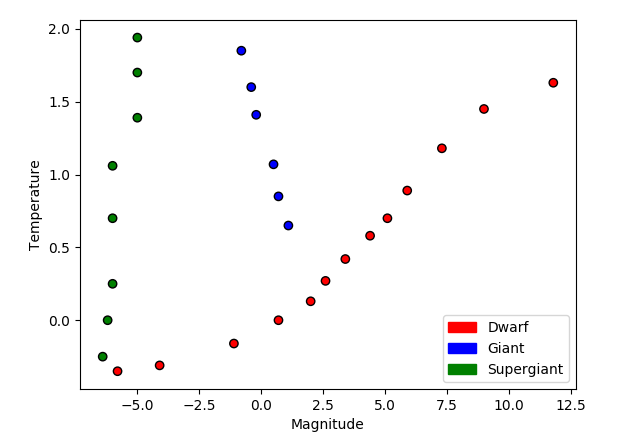
\includegraphics[width=.5\textwidth]{images/star.png}
\end{center}

Please implement the following classifiers in the \verb|SoftmaxRegression| and \verb|KNNClassifier| classes:

\begin{enumerate}[label=\alph*)]

\item \textbf{A generative classifier with Gaussian class-conditional
  densities with a \textit{shared covariance} matrix} across all classes. 
  Feel free to re-use your Problem 2 results.

\item \textbf{Another generative classifier with Gaussian class-conditional densities , but now 
with a \textit{separate covariance} matrix} learned for each class. (Note: 
The staff implementation can switch between the two Gaussian generative classifiers with just a
few lines of code.)

\item \textbf{A multi-class logistic regression classifier} using the softmax activation function. In your implementation of gradient descent, \textbf{make sure to include a bias term and use L2 regularization} with regularization parameter $\lambda = 0.001$. Limit the number of iterations of gradient descent to 200,000, and set the learning rate to be $\eta = 0.001$.

\item \textbf{Another multi-class logistic regression classifier} with feature map $\phi(\boldx) = [\ln (x_1 + 10), x_2^2]^\top$, where $x_1$ and $x_2$ represent the values for magnitude and temperature, respectively.

\item \textbf{A kNN classifier} in which you classify based on the $k = 1$ and $k = 5$ nearest neighbors and the following distance function: $$dist(star_1, star_2) = (mag_1 - mag_2)^2/9 + (temp_1 - temp_2)^2$$
where nearest neighbors are those with the smallest distances from a given point.

  Note 1: When there are more than two labels, no label may have the
  majority of neighbors.  Use the label that has the most votes among
  the neighbors as the choice of label. 

  Note 2: The grid of points for which you are making predictions
  should be interpreted as our test space.  Thus, it is not necessary
  to make a test point that happens to be on top of a training point
  ignore itself when selecting neighbors.

\end{enumerate}

After implementing the above classifiers, complete the following exercises:

\begin{enumerate}
    \item Plot the decision boundaries generated by each classifier for the dataset. Include them in your PDF. 
    Identify the similarities and differences among the classifiers. What explains the differences---in particular, which aspects or properties of each model dictate the shape of its decision boundary? 
    
    \item 
    
    Consider a star with Magnitude 3 and Temperature -2. To which class does each classifier assign this star? Report the classification probabilities of this star for each model. 
    
    Interpret how each model makes its classification decision. What are the pros and cons of each interpretation? What else should we, the modelers, be aware of when making predictions on a test point ``far" from our training data? \textbf{Your response should no be longer than 5 sentences.}
\end{enumerate}
\end{problem}

%%%%%%%%%%%%%%%%%%%%%%%%%%%%%%%%%%%%%%%%%%%%%
% Name and Calibration
%%%%%%%%%%%%%%%%%%%%%%%%%%%%%%%%%%%%%%%%%%%%%
\subsection*{Name}

\subsection*{Collaborators and Resources}
Whom did you work with, and did you use any resources beyond cs181-textbook and your notes?


\end{document}
